% Autor: Alfredo Sánchez Alberca (asalber@ceu.es)

\newproblem{ext-1}{gen}{*}
%ENUNCIADO
{La figura adjunta es la de la derivada de una función.  Estudiar el comportamiento de la función (crecimiento, decrecimiento, extremos, concavidad y convexidad).
\[
% Author: Alfredo Sánchez Alberca (asalber@ceu.es)
\begin{tikzpicture}
\begin{axis}[
    scale only axis,
    axis x line=middle,
    axis y line=left,
    xlabel={$x$},
    ylabel={$y$},
    every axis x label/.style={at={(ticklabel* cs:1)}, anchor=west,},
	every axis y label/.style={at={(ticklabel* cs:1)}, anchor=south,},
	ymin=-3, ymax=3,
    xtick={1.64, 2.41, 3.47, 4.46, 5.19},
    xticklabels={$a$, $b$, $c$, $d$, $e$},
 	xticklabel style={yshift=-3ex, anchor=south},
    height=5cm,
    yticklabels={,,}
    ]
    \addplot[domain=-0.62:8.56, samples=200, smooth, mark=none, color1] {1.7+3*(x-2)-4.3*(x-2)^2+(x-2)^3} node[anchor=south] {$f'(x)$};
\end{axis}
\end{tikzpicture}

\]
}
%SOLUCIÓN
{Crecimiento: Decreciente en $(-\infty,a)$ y $(c,e)$, y creciente en $(a,c)$ y $(e,\infty)$.\\
Extremos: Mínimos en $x=a$ y $x=e$, y máximo en $x=c$.\\
Concavidad: Cóncava en $(-\infty,b)$ y $(d,\infty)$, y convexa en $(b,d)$.
}
%RESOLUCIÓN
{
}

\newproblem{ext-2}{gen}{}
%ENUNCIADO
{Hallar $a$, $b$ y $c$ en la función  $f(x)=x^3+bx^2+cx+d$ para que tenga un punto de inflexión en $x=3$, pase por el punto $(1,0)$ y alcance un máximo en $x=1$.
}
%SOLUCIÓN
{$b=-9$, $c=15$ y $d=-7$.
}
%RESOLUCIÓN
{
}

\newproblem{ext-3}{far}{}
{Se ha diseñado un envoltorio cilíndrico para unas cápsulas. Si el contenido de las cápsulas debe ser de $0.15$ ml, hallar las dimensiones del cilindro para que el material empleado en el envoltorio sea mínimo.
}
%SOLUCIÓN
{Radio $0.2879$ cm y altura $0.5760$ cm.
}
%RESOLUCIÓN
{
}


\newproblem*{ext-4}{gen}{*}
%ENUNCIADO
{La variable aleatoria bidimensional $(X,Y)$ con función de densidad
\[
f(x,y) = \frac{1}{\sqrt{2\pi}\, \sigma_x\sigma_y} e^{-\frac{1}{2}\left(\frac{(x-\mu_x)^2}{\sigma_x^2}+\frac{(y-\mu_y)^2}{\sigma_y^2}\right)}
\]
se conoce como normal bidimensional con $X$ e $Y$ independientes, de parámetros $\mathbf{\mu}=(\mu_x,\mu_y)$ y $\mathbf{\sigma}=(\sigma_x,\sigma_y)$.
Calcular los puntos de inflexión de la curva formada por la intersección de la superficie de $f$ con el plano $y=x$.
}


\newproblem{ext-5}{amb}{*}
%ENUNCIADO
{Mediante simulación por ordenador se ha podido cuantificar la cantidad de agua almacenada en un acuífero en función del tiempo, $m(t)$, en millones de metros cúbicos, y el tiempo $t$ en años transcurridos desde el instante en el que se ha hecho la simulación, teniendo en cuenta que la ecuación sólo tiene sentido para los $t$ mayores que 0:
\[
m(t) = 10 + \frac{{\sqrt t }} {{e^t }}
\]
\begin{enumerate}
\item En el límite, cuando $t$ tiende a infinito, qué cantidad de agua almacenada habrá en el acuífero?
\item Mediante derivadas, calcular el valor del tiempo en el que el agua almacenada ser máxima y cuál es su cantidad de agua correspondiente en millones de metros cúbicos.
\end{enumerate}
}
%SOLUCIÓN
{\begin{enumerate}
\item $\lim_{t\rightarrow \infty}m(t) = 10$.
\item $\frac{dm}{dt}=e^{-t}(\frac{1}{2}t^{-1/2}-t^{1/2})$. El instante en el que el agua almacenada será máxima es $t=0.5$ años y en dicho
instante habrá $10.429$ millones de m$^3$.
\end{enumerate}
}
%RESOLUCIÓN
{
}


\newproblem{ext-6}{far}{*}
%ENUNCIADO
{Se está estudiando fabricar unas cápsulas de cuerpo cilíndrico terminadas en sus extremos por dos semiesferas. El volumen de la cápsula debe ser $0.8$ cm$^3$ y se quiere que la superficie sea mínima. ¿Cuáles deben ser las dimensiones del radio y de la longitud de la parte cilíndrica? Comentar el resultado obtenido.
\begin{quote}
    \textbf{Nota}:\\
    Volumen del cilindro $V=\pi r^2 h$\\
    Superficie lateral del cilindro $S=2\pi r h$\\
    Volumen de la esfera $V= \frac{4}{3}\pi r^3$\\
    Superficie de la esfera $S=4\pi r^2$\\
\end{quote}
}
%SOLUCIÓN
{$r = 0.5759$ y $h=0$.
}
%RESOLUCIÓN
{La capsula está formada por un cilindro de radio $r$ y altura $h$ mas una esfera (2 semiesferas) de radio $r$,
\[
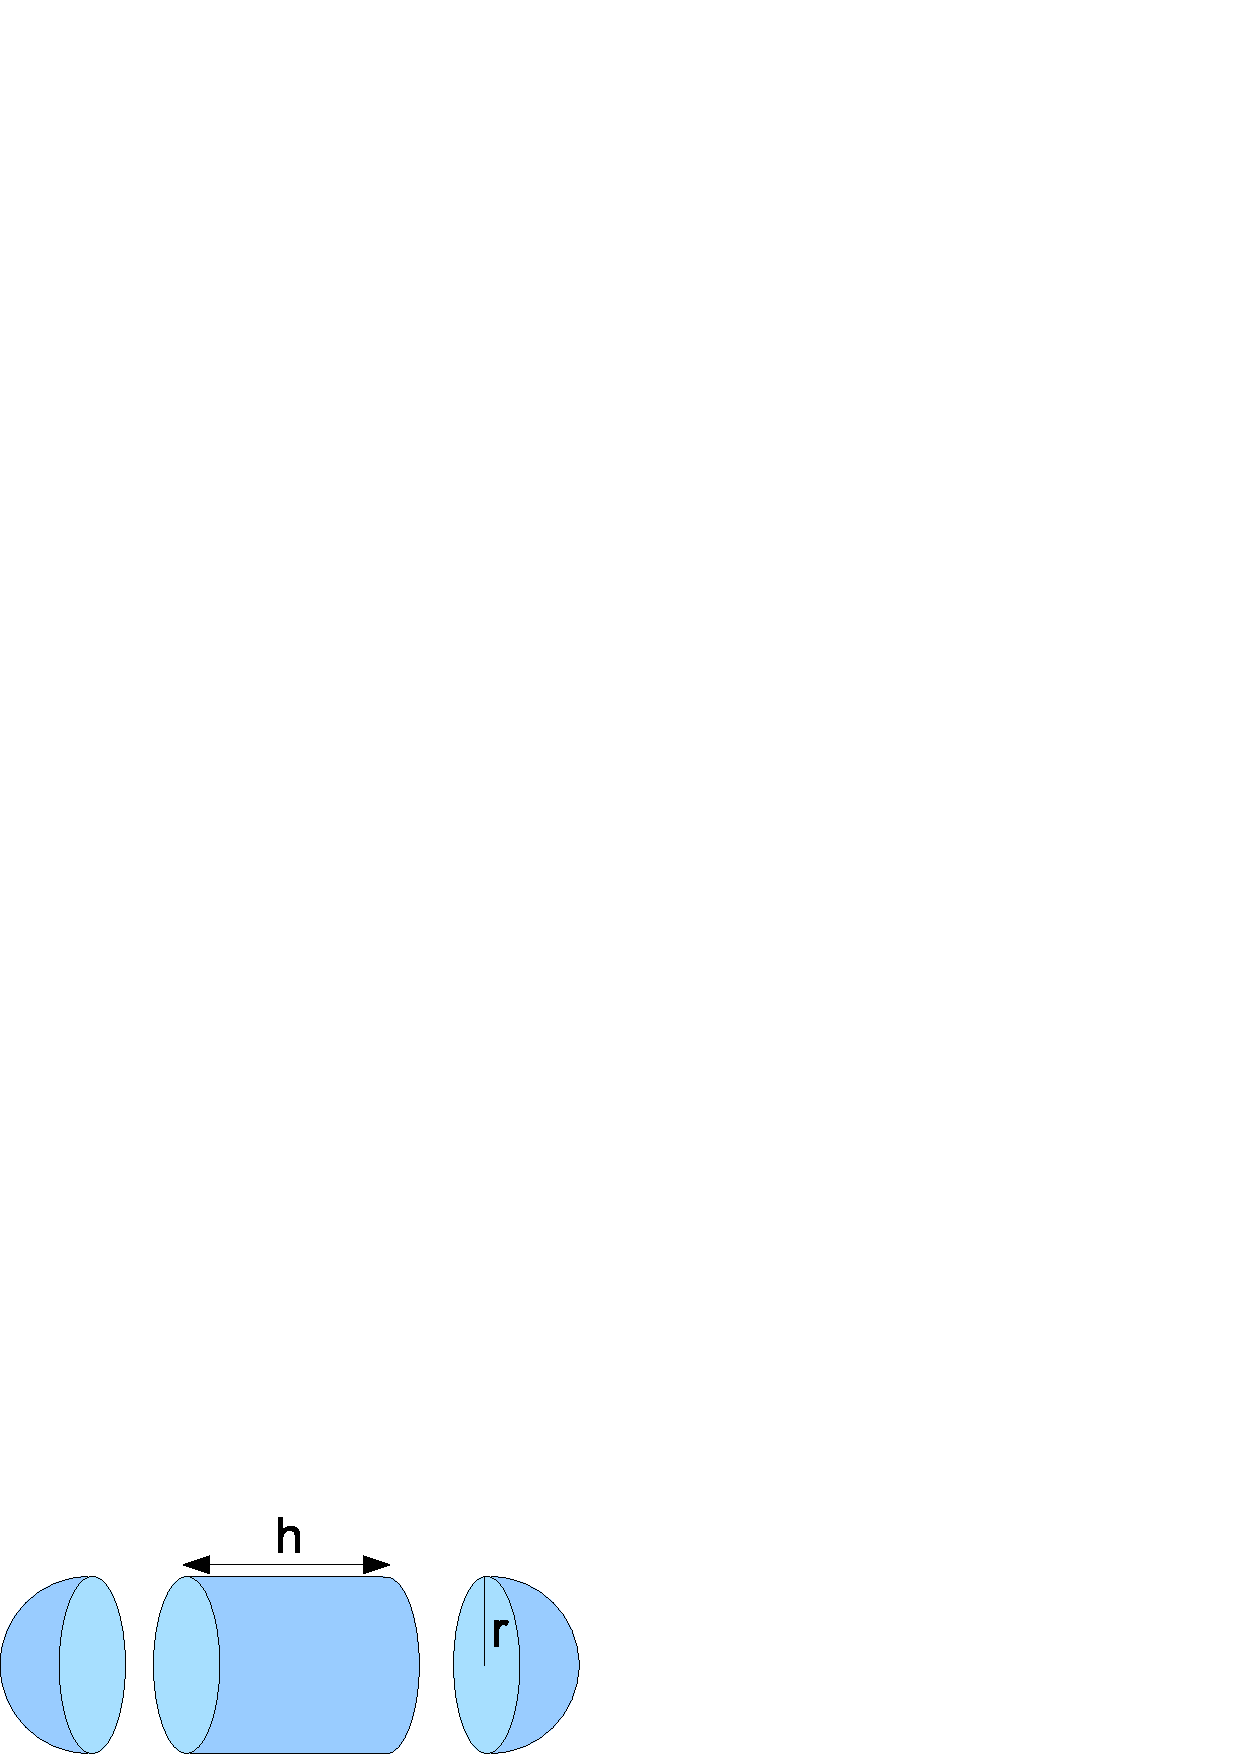
\includegraphics[scale=0.4]{img/capsula-ext-6}
\]
así que su volumen es
\[
V(r,h) = \pi r^2 h + \frac{4}{3}\pi r^3,
\]
y su superficie
\[
S(r,h) = 2\pi r h +4 \pi r^2.
\]
Como el volumen  debe ser $0.8$ cm$^3$ tenemos que
\[
V(r,h) = \pi r^2 h + \frac{4}{3}\pi r^3 = 0.8 \Leftrightarrow h = \frac{0.8-4/3\pi r^3}{\pi r^2},
\]
y sustituyendo en la fórmula de superficie tenemos
\[
S(r) = 2\pi r \frac{0.8-4/3 \pi r^3}{\pi r^2} +4 \pi r^2 = \frac{1.6-8/3\pi r^2}{r}+4\pi r^2 = \frac{1.6}{r}-\frac{8}{3}\pi r^2 +4\pi r^2 = \frac{1.6}{r^2}+\frac{4}{3}\pi r^2
\]
Como queremos que la superficie de la cápsula sea mínima, tenemos que buscar el mínimo de esta función. Para ello, calculamos primero los puntos críticos que anulan su derivada:
\[
\frac{dS}{dr} = -\frac{1.6}{r^2}+\frac{4}{3}\pi2r = 0 \Leftrightarrow \frac{1.6}{r^2} = \frac{8}{3}\pi r \Leftrightarrow \frac{8}{3}\pi r^3 = 1.6 \Leftrightarrow r^3 = \frac{1.6}{8/3 \pi} = 0.1910 \Leftrightarrow r = \sqrt[3]{0.1910} = 0.5759
\]
y por tanto la altura será
\[
h = \frac{0.8-4/3\pi r^3}{\pi r^2} = \frac{0.8-4/3\pi 0.5759^3}{\pi 0.5759^2} = 0.
\]
Esto quiere decir, que realmente no habría cilindro, y por tanto para que la supercie sea mínima la cápsula debería tener forma de esfera.

Sólo falta comprobar que el punto anterior es realmente un punto de mínimo. Para ello podemos utilizar la segunda derivada
\[
\frac{d^2S}{dr^2} = \frac{d}{dr}\left(-\frac{1.6}{r^2}+\frac{8}{3}\pi r\right) = \frac{1.6\cdot 2r}{r^4}+\frac{8}{3}\pi = \frac{3.2}{r^3}+\frac{8}{3}\pi.
\]
y sustituyendo en el punto anterior tenemos
\[
\frac{d^2S}{dr^2}(0.5759) =  \frac{3.2}{0.5759^3}+\frac{8}{3}\pi = 25.13 >0,
\]
que al tener signo positivo indica que efectivamente se trata de un mínimo.
}

\newproblem{ext-7}{gen}{*}
%ENUNCIADO
{Sea $f(x)$ una función cuya derivada vale:
\[
f'(x) = \frac{(2-x) e^{-\frac{x^2}{2}+2x-2}}{\sqrt{2\pi}}
\]
Se pide:
\begin{enumerate}
\item Estudiar el crecimiento de $f$.
\item Calcular los valores de $x$ en los que $f$ tiene extremos relativos.
\item Estudiar la concavidad de $f$.
\item Calcular los valores de $x$ en los que $f$ tiene puntos de inflexión.
\end{enumerate}
}
%SOLUCIÓN
{\begin{enumerate}
\item Creciente en $x<2$ y decreciente en $x>2$.
\item Máximo relativo en $x=2$.
\item Cóncava en $(-\infty,1)$ y $(3,\infty)$. Convexa en $(1,3)$.
\item Puntos de inflexión en $x=1$ y $x=3$.
\end{enumerate}
}
%RESOLUCIÓN
{
}


\newproblem{ext-8}{qui}{}
%ENUNCIADO
{La velocidad $v$ de una reacción irreversible $A+B\rightarrow AB$ es función de la concentración $x$ del producto $AB$ y puede expresarse según la ecuación
\[
v(x) = 4(3-x)(5-x).
\]
¿Qué valor de $x$ maximiza la velocidad de reacción?
}
%SOLUCIÓN
{Ninguno.
}
%RESOLUCIÓN
{
}


\newproblem{ext-9}{amb}{}
%ENUNCIADO
{La cantidad de trigo en una cosecha $C$ depende del nivel de nitrógeno en el suelo $n$ según la ecuación
\[
C(n) = \frac{n}{1+n^2},\quad n\geq 0.
\]
¿Para qué nivel de nitrógeno se obtendrá la mayor cosecha de trigo?
}
%SOLUCIÓN
{$n=1$.
}
%RESOLUCIÓN
{
}


\newproblem{ext-10}{amb}{}
%ENUNCIADO
{Existen organismos que se reproducen una sóla vez en su vida como por ejemplo los salmones.
En este tipo de especies, la velocidad de incremento per cápita $v$, que mide la capacidad reproductiva, depende de la edad $x$ según la ecuación
\[
v(x) = \frac{\log(p(x)h(x))}{x},
\]
donde $p(x)$ es la probabilidad de sobrevivir hasta la edad $x$ y $h(x)$ es el número de nacimientos de hembras a la edad $x$.
Calcular la edad óptima de reproducción, es decir, el valor que maximice $v$, para $p(x)=e^{-0.1x}$ y $h(x)=4x^{0.9}$.}
%SOLUCIÓN
{$x=0.58$ años.
}
%RESOLUCIÓN
{
}


\newproblem{ext-12}{amb}{}
%ENUNCIADO
{La sensibilidad de $S$ de un organismo ante un fármaco depende de la dosis $x$ suministrada según la relación
\[
S(x) = x(C-x),
\]
siendo $C$ la cantidad máxima del fármaco que puede suministrarse, que depende de cada individuo.
Hallar la dosis $x$ para la que la sensibilidad es máxima.
}
%SOLUCIÓNsensibilidad
{$x=C/2$.
}
%RESOLUCIÓN
{
}
